\documentclass [12pt]{article}
\usepackage{tikz,pgfplots}
\usetikzlibrary{arrows,calc}
\newenvironment{customlegend}[1][]{%
    \begingroup
    % inits/clears the lists (which might be populated from previous
    % axes):
    \csname pgfplots@init@cleared@structures\endcsname
    \pgfplotsset{#1}%
}{%
    % draws the legend:
    \csname pgfplots@createlegend\endcsname
    \endgroup
}%

% makes \addlegendimage available (typically only available within an
% axis environment):
\def\addlegendimage{\csname pgfplots@addlegendimage\endcsname}

%%--------------------------------

% definition to insert numbers
\pgfkeys{/pgfplots/number in legend/.style={%
        /pgfplots/legend image code/.code={%
            \node at (0.295,-0.0225){#1};
        },%
    },
}
%%===================================

\begin{document}


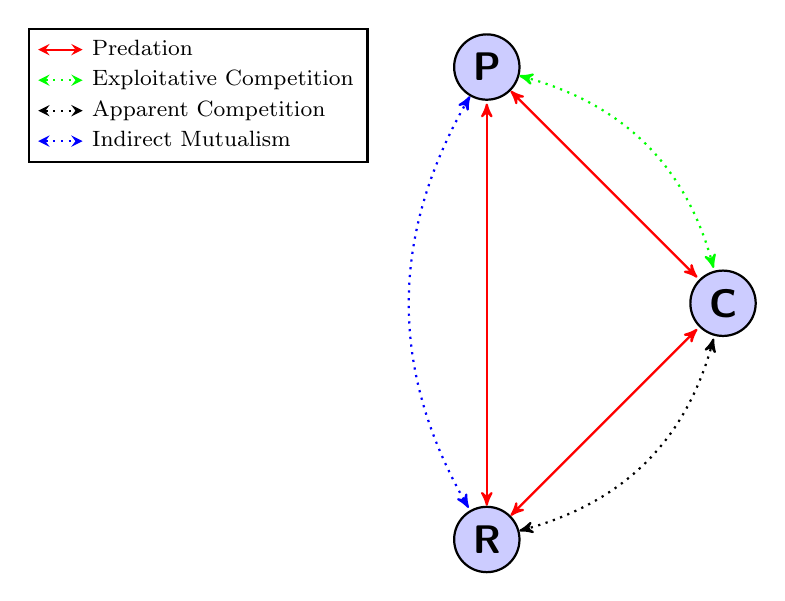
\begin{tikzpicture}[<->,>=stealth',shorten >=1pt,auto,
  thick,main node/.style={circle,fill=blue!20,draw,font=\sffamily\Large\bfseries}]


\node[main node] (R) at (0,-3){R};
\node[main node] (C) at (3,0) {C};
\node[main node] (P) at (0,3) {P};

 \path[every node/.style={font=\sffamily\small}]

(R) edge [red] (C)
(R) edge [red] (P)
(P) edge [red] (C)
(P) edge [bend right , dotted, blue] (R) 
(P) edge [bend left , dotted, green]  (C)
(R) edge [bend right ,dotted , black] (C);



\begin{customlegend}[legend cell align=left,
legend entries={ % <= in the following there are the entries
Predation,
Exploitative Competition,
Apparent Competition, 
Indirect Mutualism
},
legend style={at={(-1.5,3.5)},font=\footnotesize}] % <= to define position and font legend
% the following are the "images" and numbers in the legend
    \addlegendimage{stealth-stealth,red}
    \addlegendimage{stealth-stealth,dotted,green}
    \addlegendimage{stealth-stealth,dotted,black}
    \addlegendimage{stealth-stealth,dotted,blue}
    
\end{customlegend}

\end{tikzpicture}
\end{document}